\chapter{Towards Model-based Run-time State Migration}
\label{ch:requirements}

\section{Requirements Analysis}

A requirement analysis shall be applied to identify what approach has to offer. This includes what needs to be part of the modeling language and what has to be implemented. To solve it, as a prerequisite, we need to be able to model states, in general, to know which migratable states are involved in the application's scope. Also, we need to find at least two existing applications which are suitable to apply the approach.

\subsection{R1 Applicable on Existing Applications}
This approach shall allow adapting existing same-purpose applications, so they support run-time state migration.

\subsection{R2 State Management}
It shall be possible to model which and when parts of existing applications can be migrated. Also, it shall be possible to model these states.

\subsection{R3 Device Management and Device Discovery}
It must be possible to find, retrieve and select devices offering the same states. Also, It shall be possible to express if the application knows another application has the same state one same network.

\section{Requirements for a DSL}

\subsection{D1 Specification a State}
The DSL shall be able to provide the specification of a state by defining a model. State whose are following these specifications can be migrated between applications explicitly or implicitly.
\subsection{D2 Finding Same Model}
The DSL must allow specifying a way for finding the same model. These specifications can be a unique model name and model version.
\subsection{D3 Validating}    
The DSL must have a version to allow validating the specification of a state.



\section{Same-purpose Applications Analysis}
To show the approach's feasibility, two current existing open-source applications that are serving the same purpose shall be adapted to support run-time state migration.
These applications shall be for different platforms, and their source code should be freely accessible to allow the integration of the approach.
They shall be interactive applications for end-users and have sufficient complexity (e.g., applications should not have only one single state).

In this section, some different pair of same-purpose applications got analyzed, and we found the commons state of them.

\subsection{State Analysis of Applications}
\subsubsection{States of E-mail Applications}

Table \ref{tab:states_of_email_applications} shows a list of available states of two open-source e-mail clients. Some states can be candidates for migration, which are common in both applications.

\begin{table}[ht!]
\begin{tabular}{lll}
State / E-mail client                   & Mailspring & K-9 Mail \\
\hline
Welcome   Screen                        & \checkmark          & \checkmark        \\
Account Registration                    & \checkmark          &          \\
Account Login                           & \checkmark          &          \\
Add an e-mail service account           & \checkmark          & \checkmark        \\
Import   Settings                       &            & \checkmark        \\
Export Settings and Accounts            &            & \checkmark        \\
Settings                                & \checkmark          & \checkmark        \\
Sync New E-mails                        & \checkmark          & \checkmark        \\
Compose a   new E-email                 & \checkmark          & \checkmark        \\
Forward an E-mail                       & \checkmark          &          \\
Replay an   E-mail                      & \checkmark          & \checkmark        \\
Sending an E-mail                       & \checkmark          & \checkmark        \\
Trashing   an E-mail                    & \checkmark          & \checkmark        \\
E-mails list (Inbox, Sent, Draft, …)    & \checkmark          & \checkmark        \\
Single   E-mail                         & \checkmark          & \checkmark        \\
Show Original Version of E-mail         & \checkmark          &          \\
Search   View                           & \checkmark          & \checkmark        \\
Searching                               & \checkmark          & \checkmark        \\
Loading   E-mails                       & \checkmark          & \checkmark        \\
Loading Activity Data                   & \checkmark          &          \\
Activity   View                         & \checkmark          &          \\
Exporting Activity Data                 & \checkmark          &          \\
Sharing   Report of Activity Data       & \checkmark          &          \\
Marking Star/Spam/Read/Unread an E-mail & \checkmark          & \checkmark       
\end{tabular}
\caption{States of E-mail Applications}
\label{tab:states_of_email_applications}
\end{table}

\newpage
\subsubsection{States of Browsers}

Table \ref{tab:state_browsers} shows a list of available states of two browser applications. Some states can be candidates for migration, which are common in both applications. 

Some states information are form official Chrome Page lifecycle API\footnote{\href{https://developers.google.com/web/updates/2018/07/page-lifecycle-api}{https://developers.google.com/web/updates/2018/07/page-lifecycle-api}} and Mozilla Web API\footnote{\href{https://developer.mozilla.org/en-US/docs/Web/API}{https://developer.mozilla.org/en-US/docs/Web/API}}. Also, For browsers there is a standard called W3C Page lifecycle API\footnote{\href{https://wicg.github.io/page-lifecycle/}{https://wicg.github.io/page-lifecycle/}}.


\begin{table}[ht!]
\begin{tabular}{lll}
State / Browser                                       & Firefox (macOS) & Chrome (Android) \\
\hline
Home page                                             & \checkmark      & \checkmark       \\
Single Tab (Preferences, Bookmarks, Performance,   …) & \checkmark      & \checkmark       \\
Extensions   Tab                                      & \checkmark      &                  \\
Syncing                                               & \checkmark      & \checkmark       \\
Browsing                                              & \checkmark      & \checkmark       \\
Current Tab                                           & \checkmark      & \checkmark       \\
Developer   Console                                   & \checkmark      &                  \\
Signing in                                            & \checkmark      & \checkmark       \\
Finding   (in page)                                   & \checkmark      & \checkmark       \\
Printing                                              & \checkmark      &                  \\
Downloading                                           & \checkmark      & \checkmark       \\
Sharing                                               &                 & \checkmark       \\
Private/Incognito   Mode                              & \checkmark      & \checkmark       \\
Light mode                                            &                 & \checkmark      
\end{tabular}
\caption{States of Browsers applications}
\label{tab:state_browsers}
\end{table}


\subsubsection{States of Video Player Applications}
Table \ref{tab:states_video_players} shows a list of available states of two video player applications. Some states can be candidates for migration, which are common in both applications. 

To support run-time state migration on video players, we needed to access the video file, considering the video's size is not the right choice. However, run-time state migration can be supported on video streaming applications with the same media.

\begin{table}[ht!]
\begin{tabular}{lll}
State / Video Player                                               & IINA (macOS) & VLC (Android) \\
\hline
Welcome   Screen                                                   & \checkmark       & \checkmark        \\
Video player tips                                                  &              & \checkmark        \\
Audio   player tips                                                &              & \checkmark        \\
Pause                                                              & \checkmark       & \checkmark        \\
Deleting                                                           &              & \checkmark        \\
Browsing view                                                      & \checkmark       & \checkmark        \\
Loading   Directories                                              &              & \checkmark        \\
Single Page view (About, Settings, Audio,   Video, …) & \checkmark       & \checkmark        \\
Search   result                                                    &              & \checkmark        \\
Searching                                                          &              & \checkmark        \\
Playing   video                                                    & \checkmark       & \checkmark        \\
Playing audio                                                      & \checkmark       &               \\
Showing   picture                                                  & \checkmark       &               \\
Streaming                                                          & \checkmark       & \checkmark        \\
Loading   local network devices                                    &              & \checkmark       
\end{tabular}
\caption{States of Video player applications}
\label{tab:states_video_players}
\end{table}

\newpage
\subsubsection{States of Note Taking Applications}
Table \ref{tab:states_note_apps} shows a list of available states of two note-taking applications. Some states can be candidates for migration, which are common in both applications. 


\begin{table}[ht!]
\begin{tabular}{lll}
State / Note taking application                                          & Laverna (macOS) & Joplin (Android) \\
\hline
Loading   Screen                                                         & \checkmark          &                  \\
Welcome Screen                                                           & \checkmark          &                  \\
Encryption   view                                                        & \checkmark          &                  \\
Syncing on Cloud                                                         & \checkmark          & \checkmark           \\
Importing   and Exporting settings                                       & \checkmark          &                  \\
Importing and Exporting data                                             & \checkmark          & \checkmark           \\
Single   Page view (All notes, Favorites, Settings, ...) & \checkmark          & \checkmark           \\
Search                                                                   & \checkmark          & \checkmark           \\
Searching                                                                & \checkmark          & \checkmark           \\
Writing a Note                                                           & \checkmark          & \checkmark           \\
Writing a   Todo                                                         &                 & \checkmark           \\
Saving a Note                                                            & \checkmark          & \checkmark           \\
Note   Properties                                                        &                 & \checkmark           \\
New Notebook                                                             & \checkmark          & \checkmark           \\
New Tags                                                                 & \checkmark          & \checkmark           \\
Share view                                                               &                 & \checkmark           \\
Trashing                                                                 & \checkmark          &                  \\
Removing                                                                 & \checkmark          &                 
\end{tabular}
\caption{States of Note taking applications}
\label{tab:states_note_apps}
\end{table}

\section{Modeling States}
To check the feasibility of modeling the states, the source code of two applications is analyzed and modeled in tables. These applications are two open-source e-mail clients from two different platforms which they are \textbf{Mailspring} \footnote{\href{https://github.com/Foundry376/Mailspring}{https://github.com/Foundry376/Mailspring}} and \textbf{K-9 Mail} \footnote{\href{https://github.com/k9mail/k-9}{https://github.com/k9mail/k-9}}. 

\subsubsection{Modeling States of E-mail Applications}

\begin{table}[ht!]
\begin{tabular}{lll}
Field     & Type      & Example/Description                                    \\
\hline
id        & String/Id & pYkSAMPpfU9bU1E33219fbaJyVoQ71hS8Vvs7gDZC              \\
aid       & String/Id & 0a6dbf86                                               \\
v         & Number    & 3                                                      \\
metadata  & Array     & Information   About Mail/Link tracking                 \\
to        & Array     & []                                                     \\
cc        & Array     & []                                                     \\
bcc       & Array     & []                                                     \\
from      & Array     & []                                                     \\
replyto   & Array     & []                                                     \\
date      & Number    & 1595782508                                             \\
body      & String    & <div>This is a test   body</div><br/>                  \\
files     & Array     & []                                                     \\
unread    & Boolean   & False                                                  \\
events    & Array     & []                                                     \\
starred   & Boolean   & False                                                  \\
threadid  & String/Id & “”                                                     \\
subject   & String    & Test   Subject                                         \\
draft     & Boolean   & True                                                   \\
pristine  & Boolean   & False                                                  \\
plaintext & Boolean   & False                                                  \\
folder    & Object    & {}                                                     \\
"file\_ids"  & Array  & []                                                  \\
object    & String    & “draft”                                               
\end{tabular}
\caption{Modeling the State: Compose a new Email in Mailspring}
\label{tab:compose_new_email_mailspring}
\end{table}


% \newpage
\begin{table}[ht!]
\begin{tabular}{lll}
Field     & Type      & Example/Description \\
\hline
\_ID            & String &  \\
SEND\_DATE      & String     &                     \\
SENDER         &  String    &                     \\
SUBJECT        &  String    &                     \\
PREVIEW        &  String    &                     \\
ACCOUNT        &   String   &                     \\
DELETE\_URI     &  String    &                     \\
SENDER\_ADDRESS &   String   &                    
\end{tabular}
\caption{Modeling the State: Compose a new Email in K-9 Mail}
\label{tab:compose_new_email_k9}
\end{table}


\begin{table}[ht!]
\begin{tabular}{lll}
Field       & Type    & Example/Description \\
\hline
isSearching & Boolean & False               \\
query       & String  & “master   thesis”  
\end{tabular}
\caption{Modeling the State: Search in Mailspring}
\label{tab:search_mailspring}
\end{table}


\begin{table}[ht!]
\begin{tabular}{lll}
Field & Type   & Example/Description \\
\hline
query & String & “master thesis”    
\end{tabular}
\caption{Modeling the State: Search in K-9 Mail}
\label{tab:search-k9}
\end{table}

\section{Solution Overview}
This section provides an overview of the approach and explains how it addresses requirements R1 to R3.
A visualization of the approach is shown in Fig. \ref{fig:solution-overview}. As mentioned in Requirement R1, the approach shall apply to existing applications, and they should be able to support run-time state migration. For ease of enabling existing applications, we chose to develop the necessary library. This library shall provide an API for validation, injection, and extraction states. As stated in \textbf{Requirement R2}, the approach shall enable the ability of state management. Thereby, modeling the state as state specification is possible by DSL, which will be integrated with the library.

Besides libraries, our approach needs device management and device discovery, stated in \textbf{Requirement R3}. Middleware serves as device management, allowing devices to introduce themselves and allows devices to find each other and get noticed when a device joined or left. Also, if devices are in the same local network, these libraries establish a point-to-point connection. Otherwise, they use middleware to communicate over the internet to migrate the run-time state.

Since the focus of the thesis is not providing different types of communications, only one of these communication styles is implemented.

\FloatBarrier
\begin{figure}[!b]
    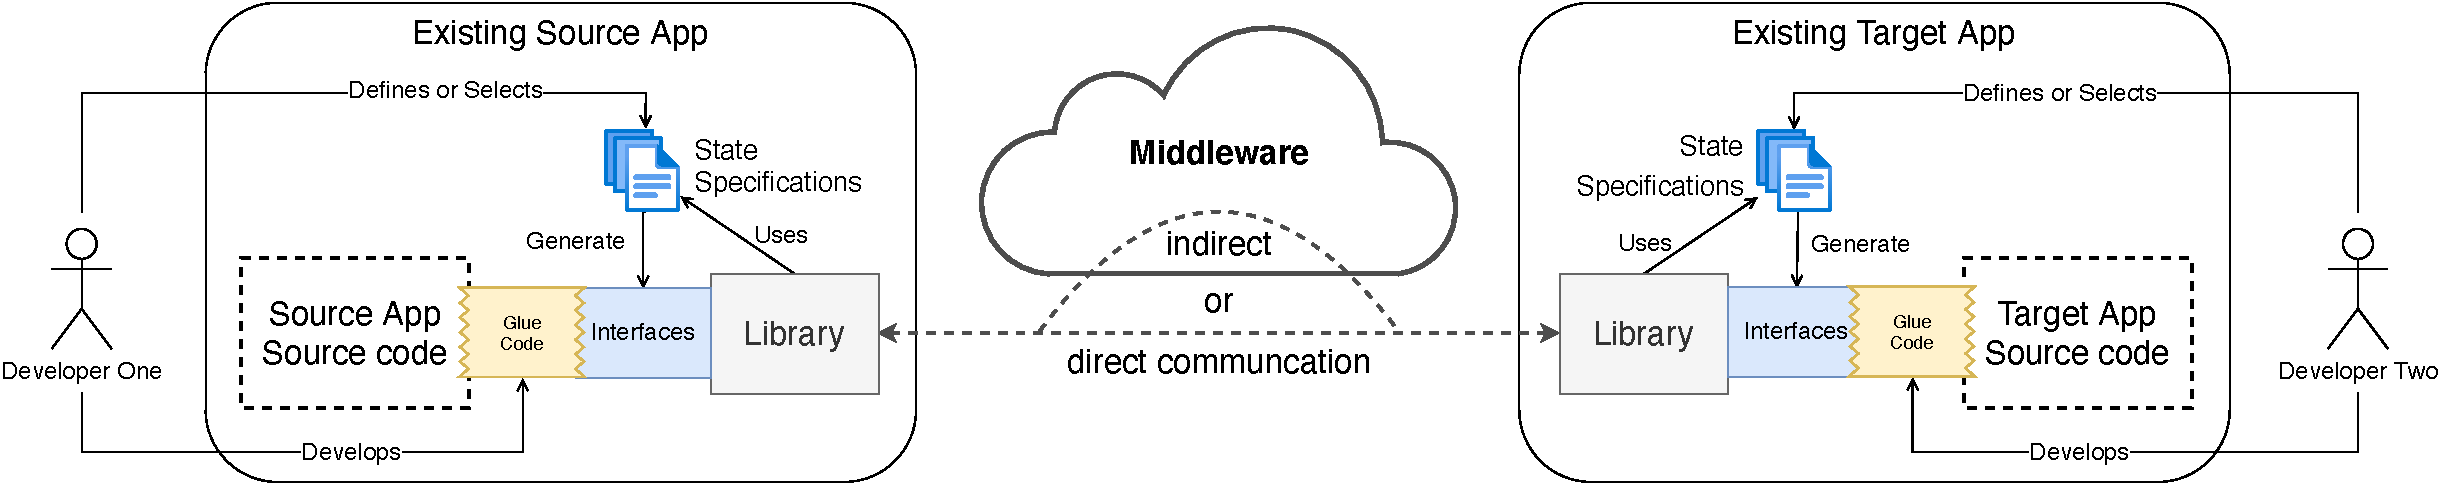
\includegraphics[width=\linewidth]{../figures/solution-overview}
    \centering
    \caption{General overview of the approach}
    \label{fig:solution-overview}
\end{figure}
\FloatBarrier